\begin{figure*}[h!]
\centering

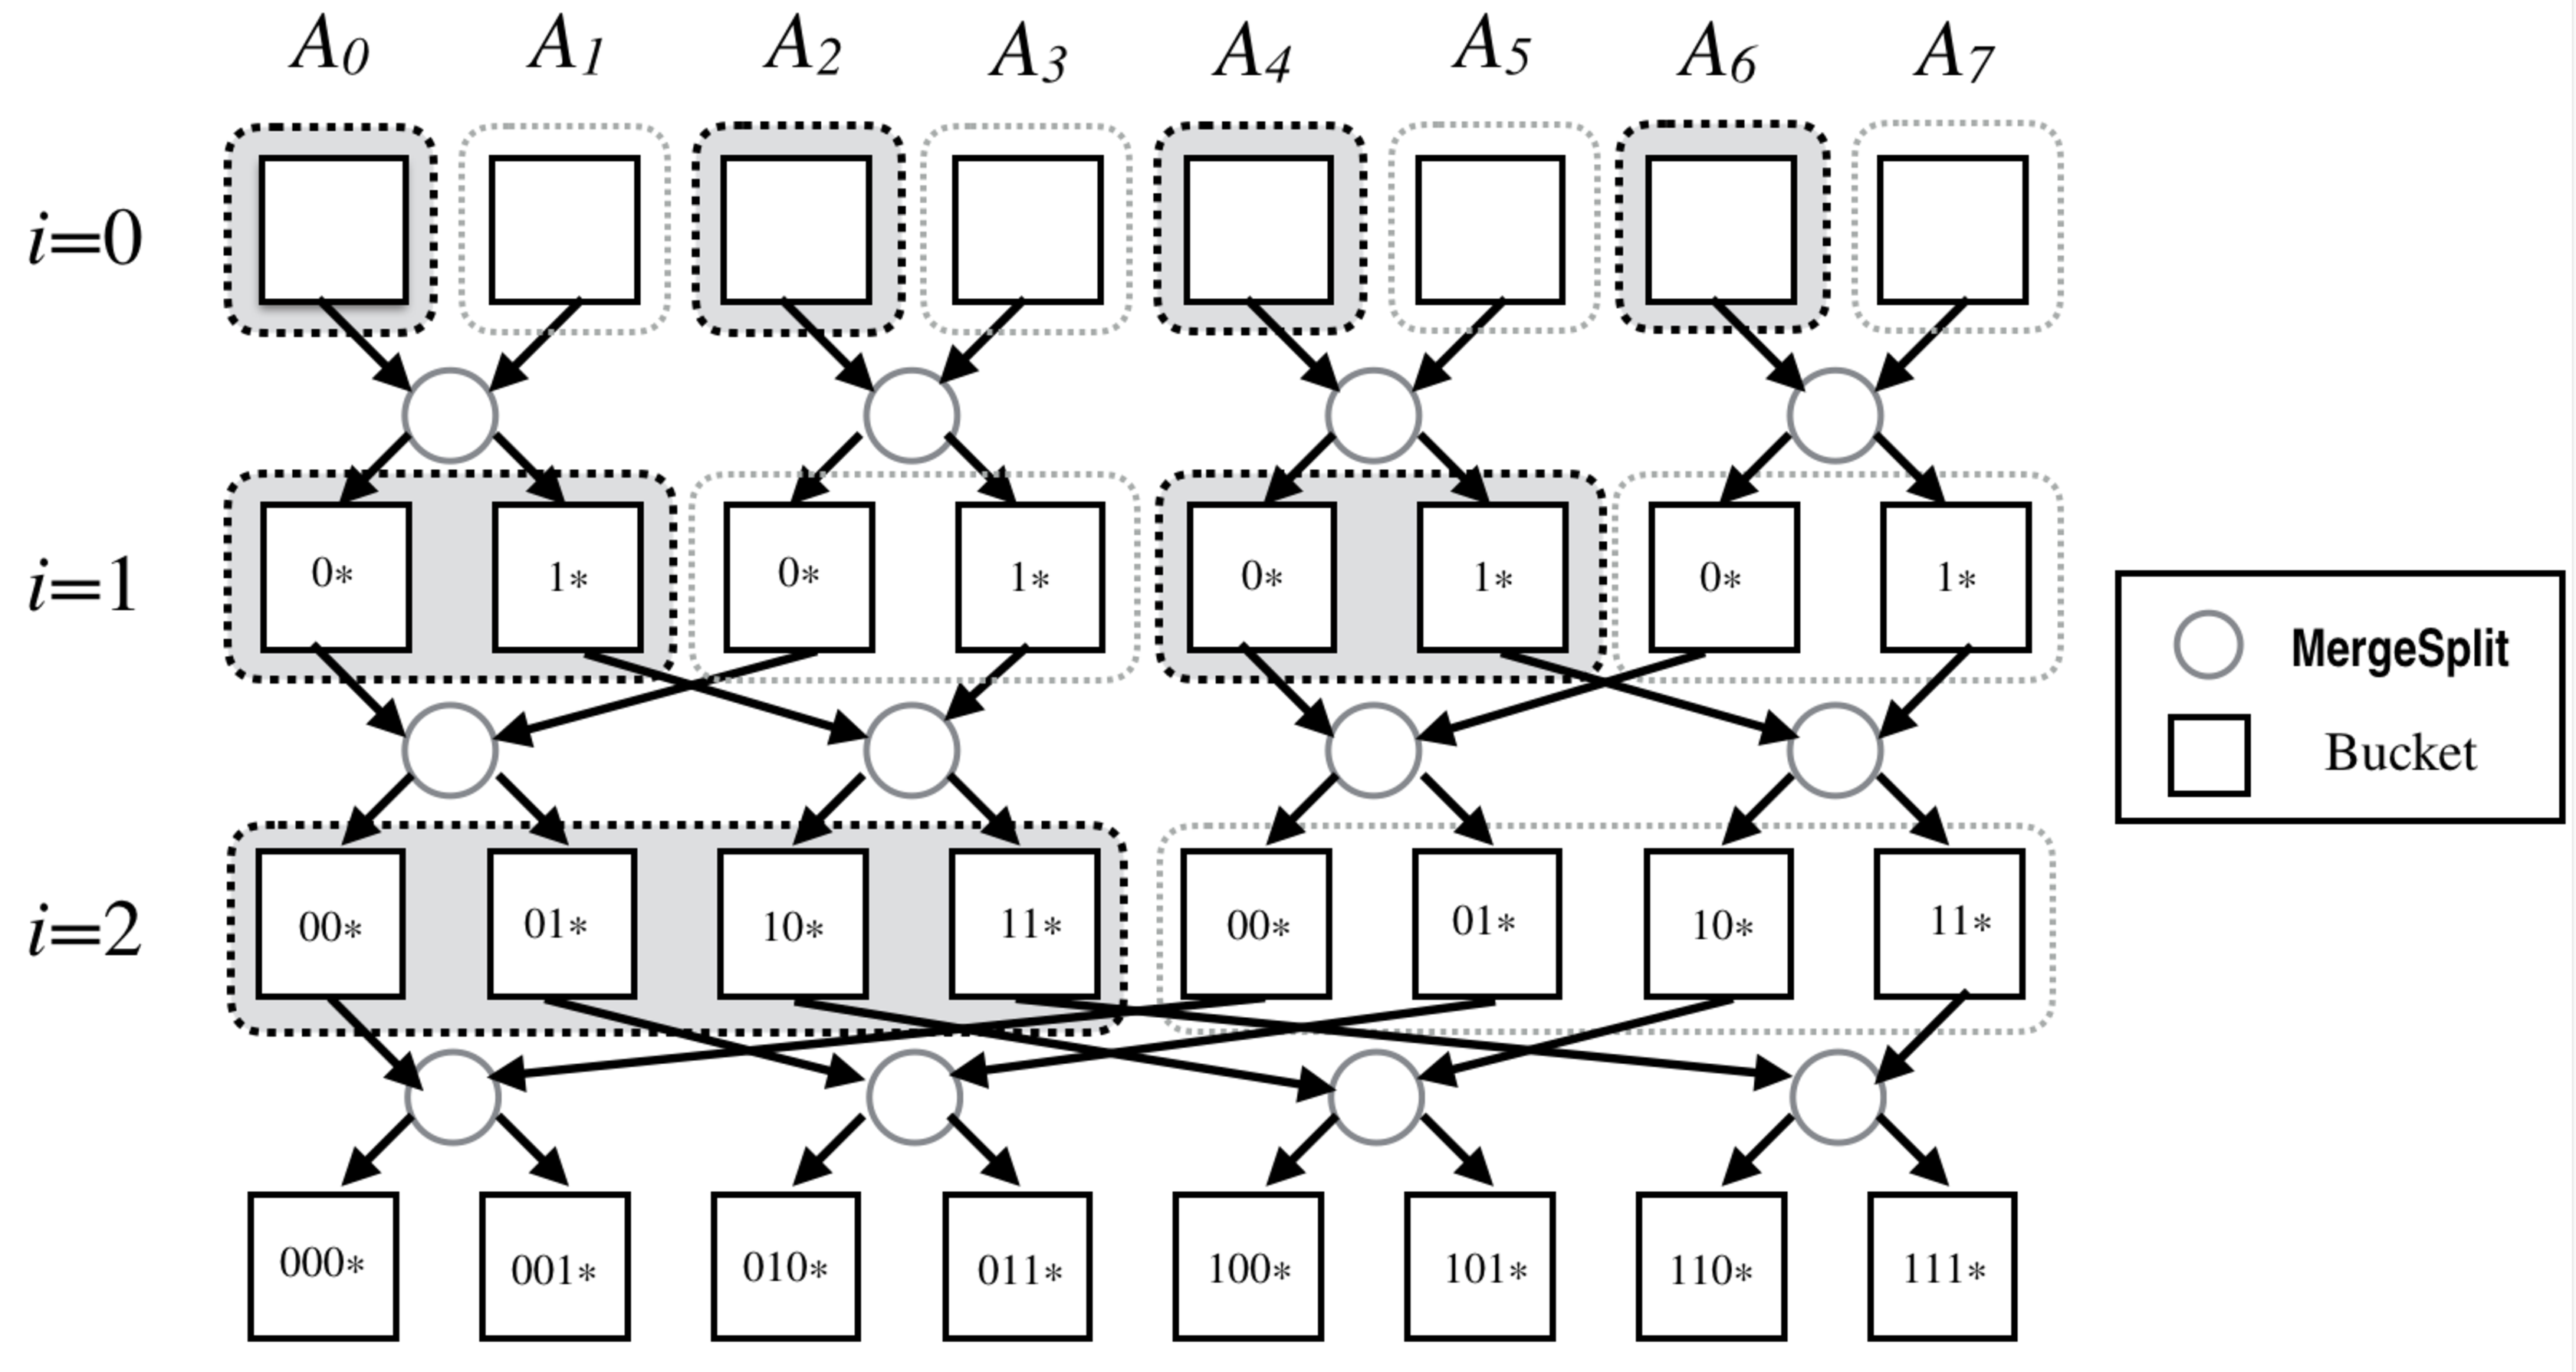
\includegraphics[width=0.7\textwidth]{RadixBucketSort1.pdf}
\captionof{figure}{Oblivious random bin assignment with 8 buckets.}
%The \textsc{MergeSplit} procedure takes elements from two buckets at level $i$ and put them into two buckets at level $i+1$, according to the $(i+1)$-th most significant bit of the keys. 
%At level $i$, every $2^{i}$ consecutive buckets are semi-sorted by the most significant $i$ bits of the keys.
\label{fig:radix-sort}

\bigskip
\begin{algorithm}[Oblivious Random Bin Assignment]
\begin{algorithmic}
\State
\State \textbf{Input}: an array $\X$ of size $n$
\State Choose a bucket size $Z$ and let $B$ be the smallest power of two that is $\geq 2n/Z$. 
\State Define $(\log B+1)$ arrays, each containing $B$ buckets of size $Z$. Denote the $j$-th bucket of the $i$-th array $A_j^{(i)}$.
\State For each element in $\X$, assign a uniformly random key in $[0,B-1]$.
\State Evenly divide $\X$ into $B$ groups. Put the $j$-th group into $A_j^{(0)}$ and pad with dummy elements to have size $Z$.

\For {$i=0,\ldots,\log B-1$}
    \For {$j=0,\ldots,B/2$}
        \State $(A^{(i+1)}_{2j}, A^{(i+1)}_{2j+1}) \leftarrow \textsc{MergeSplit}(A^{(i)}_{j'+j}, A^{(i)}_{j'+j+2^i}, i)$ where $j'=\lfloor j / {2^i} \rfloor \cdot 2^{i+1}$
        \State \Comment{Input: $j$-th pair of buckets with distance $2^i$ in $A^{(i)}$; Output: $j$-th pair of buckets in $A^{(i+1)}$}
        %\State Let $(A_0, A_1$) be the $j$-th pair of buckets with distance $2^i$ in $A^{(i)}$ 
        %\State Let $(A'_0, A'_1)$ be the $j$-th pair of buckets in $A^{(i+1)}$
        %\State $(A'_0, A'_1) \leftarrow \textsc{MergeSplit}(A_0, A_1, i)$ 
        
    \EndFor
\EndFor    
\State \textbf{Output:} $A^{(\log B)}$

\medskip
\Function{$(A'_0, A'_1) \leftarrow$ MergeSplit}{$A_0, A_1, i$}
    \State $A'_0$ receives all real elements in $A_0 \cup A_1$ where the $(i+1)$-st MSB of the key is $0$   
    \State $A'_1$ receives all real elements in $A_0 \cup A_1$ where the $(i+1)$-st MSB of the key is $1$
    \State If either $A'_0$ or $A'_1$ receives more than $Z$ real elements, the procedure aborts with {\sf overflow}
    \State Pad $A'_0$ and $A'_1$ to size $Z$ with dummy elements and return $(A'_0, A'_1)$
\EndFunction   
\end{algorithmic}
\label{code:obin}
\end{algorithm}

\bigskip
%\begin{table*}[t]
\centering
\begin{tabular}{|c|c|c|c|c|}
    \hline
    Algorithm & Oblivious & Client storage & Runtime & Error probability \\
    \hline
    Merge sort & no & $O(1)$ & $2n \log n$ & 0 \\
    Bitonic sort & yes & $O(1)$ & $n\log^2 n$ & 0 \\
    AKS sort~\cite{aks} & yes & $O(1)$ & $5.4\times10^7 \times n\log n$ & 0 \\
    Zig-zag sort~\cite{zigzag} & yes & $O(1)$ & $8\times10^4 \times n\log n$ & 0 \\
    Randomized Shellsort~\cite{RandShellsort} & yes & $O(1)$ & $24n\log n$ & $\approx n^{-3}$ \\
    \hline
    \textbf{Bucket oblivious sort} & yes & $2Z$ & $6 n\log n$ & $\approx e^{-Z/6}$\\
    \textbf{Bucket oblivious sort} & yes & $O(1)$ & $2n\log n \log^2 Z$ & $\approx e^{-Z/6}$ \\
    \hline   
\end{tabular}
\captionof{table}{\textbf{Runtime of bucket oblivious sort and
    classic non-oblivious and oblivious sort algorithms.} Bitonic
sort requires $\frac 14 n \log^2 n$ comparisons. Values for AKS
sort and Zig-zag sort are taken from \cite{zigzag}. Runtime
represents the number of memory accesses, which is four times the
number of comparisons.}
\label{tab:compare}
%\end{table*}

\end{figure*}
%%% Local Variables:
%%% mode: latex
%%% TeX-master: "main"
%%% End:
